%%% template.tex
%%%
%%% This LaTeX source document can be used as the basis for your technical
%%% paper or abstract. Intentionally stripped of annotation, the parameters
%%% and commands should be adjusted for your particular paper - title, 
%%% author, article DOI, etc.
%%% The accompanying ``template.annotated.tex'' provides copious annotation
%%% for the commands and parameters found in the source document. (The code
%%% is identical in ``template.tex'' and ``template.annotated.tex.'')

\documentclass[conference]{acmsiggraph}

\usepackage{authblk}

\TOGonlineid{45678}
\TOGvolume{0}
\TOGnumber{0}
\TOGarticleDOI{1111111.2222222}
\TOGprojectURL{}
\TOGvideoURL{}
\TOGdataURL{}
\TOGcodeURL{}



\title{Tracking Objects on a Deformable Surface using Displacement and Orientation Information}

\author[1]{Zachary DeStefano\thanks{zdestefa@uci.edu}}
\author[1]{Kyle Cutler\thanks{kbcutler58@gmail.com}}
\author[1]{Gopi Meenakshisundaram\thanks{gopi.meenakshisundaram@gmail.com}}
\author[1]{Bruce Tromberg\thanks{bjtrombe@uci.edu}}
\pdfauthor{Zachary DeStefano,Kyle Cutler,Gopi Meenakshisundaram,Bruce Tromberg}
\affil[1]{University of California, Irvine}

\keywords{Tracking, Deformable Surface}

\begin{document}

%% \teaser{
%%   \includegraphics[height=1.5in]{images/sampleteaser}
%%   \caption{Spring Training 2009, Peoria, AZ.}
%% }

\maketitle



\section{Mesh Traversal Algorithms}

\subsection{Following a Deformable mesh}

Even after calibration, due to measurement error and deformability, we have a path that mostly follows the surface but there will be segments that end up lying above or below the surface. The path was still recorded on the surface and we thus want to have a visualization of where the path was located on the surface itself. We thus need a method of converting the inaccurate path in the virtual world into a path that follows the surface and shows the locations on the surface that the probe traversed. \\
\\
A path is just a series of connected segments and the mesh is just a series of triangles. Thus the input of our algorithm is a segment with a start and end point as well as the triangle where it originates and the triangles neighbors. We need to make sure the projection preserves the length of the segment. We are restricted to rotating the segment along the plane that it makes with the triangle's normal. \\
\\
We will let $v$ be the segment vector, $N$ be the normal, and $E$ be the resultant vector that is on the plane of $N$ and forms an acute angle with $v$. As can be observed in figure \ref{vectordiagram}, the following equation will then hold
\[
E + proj_N(v) = v
\]

\begin{figure}[ht]
\centering
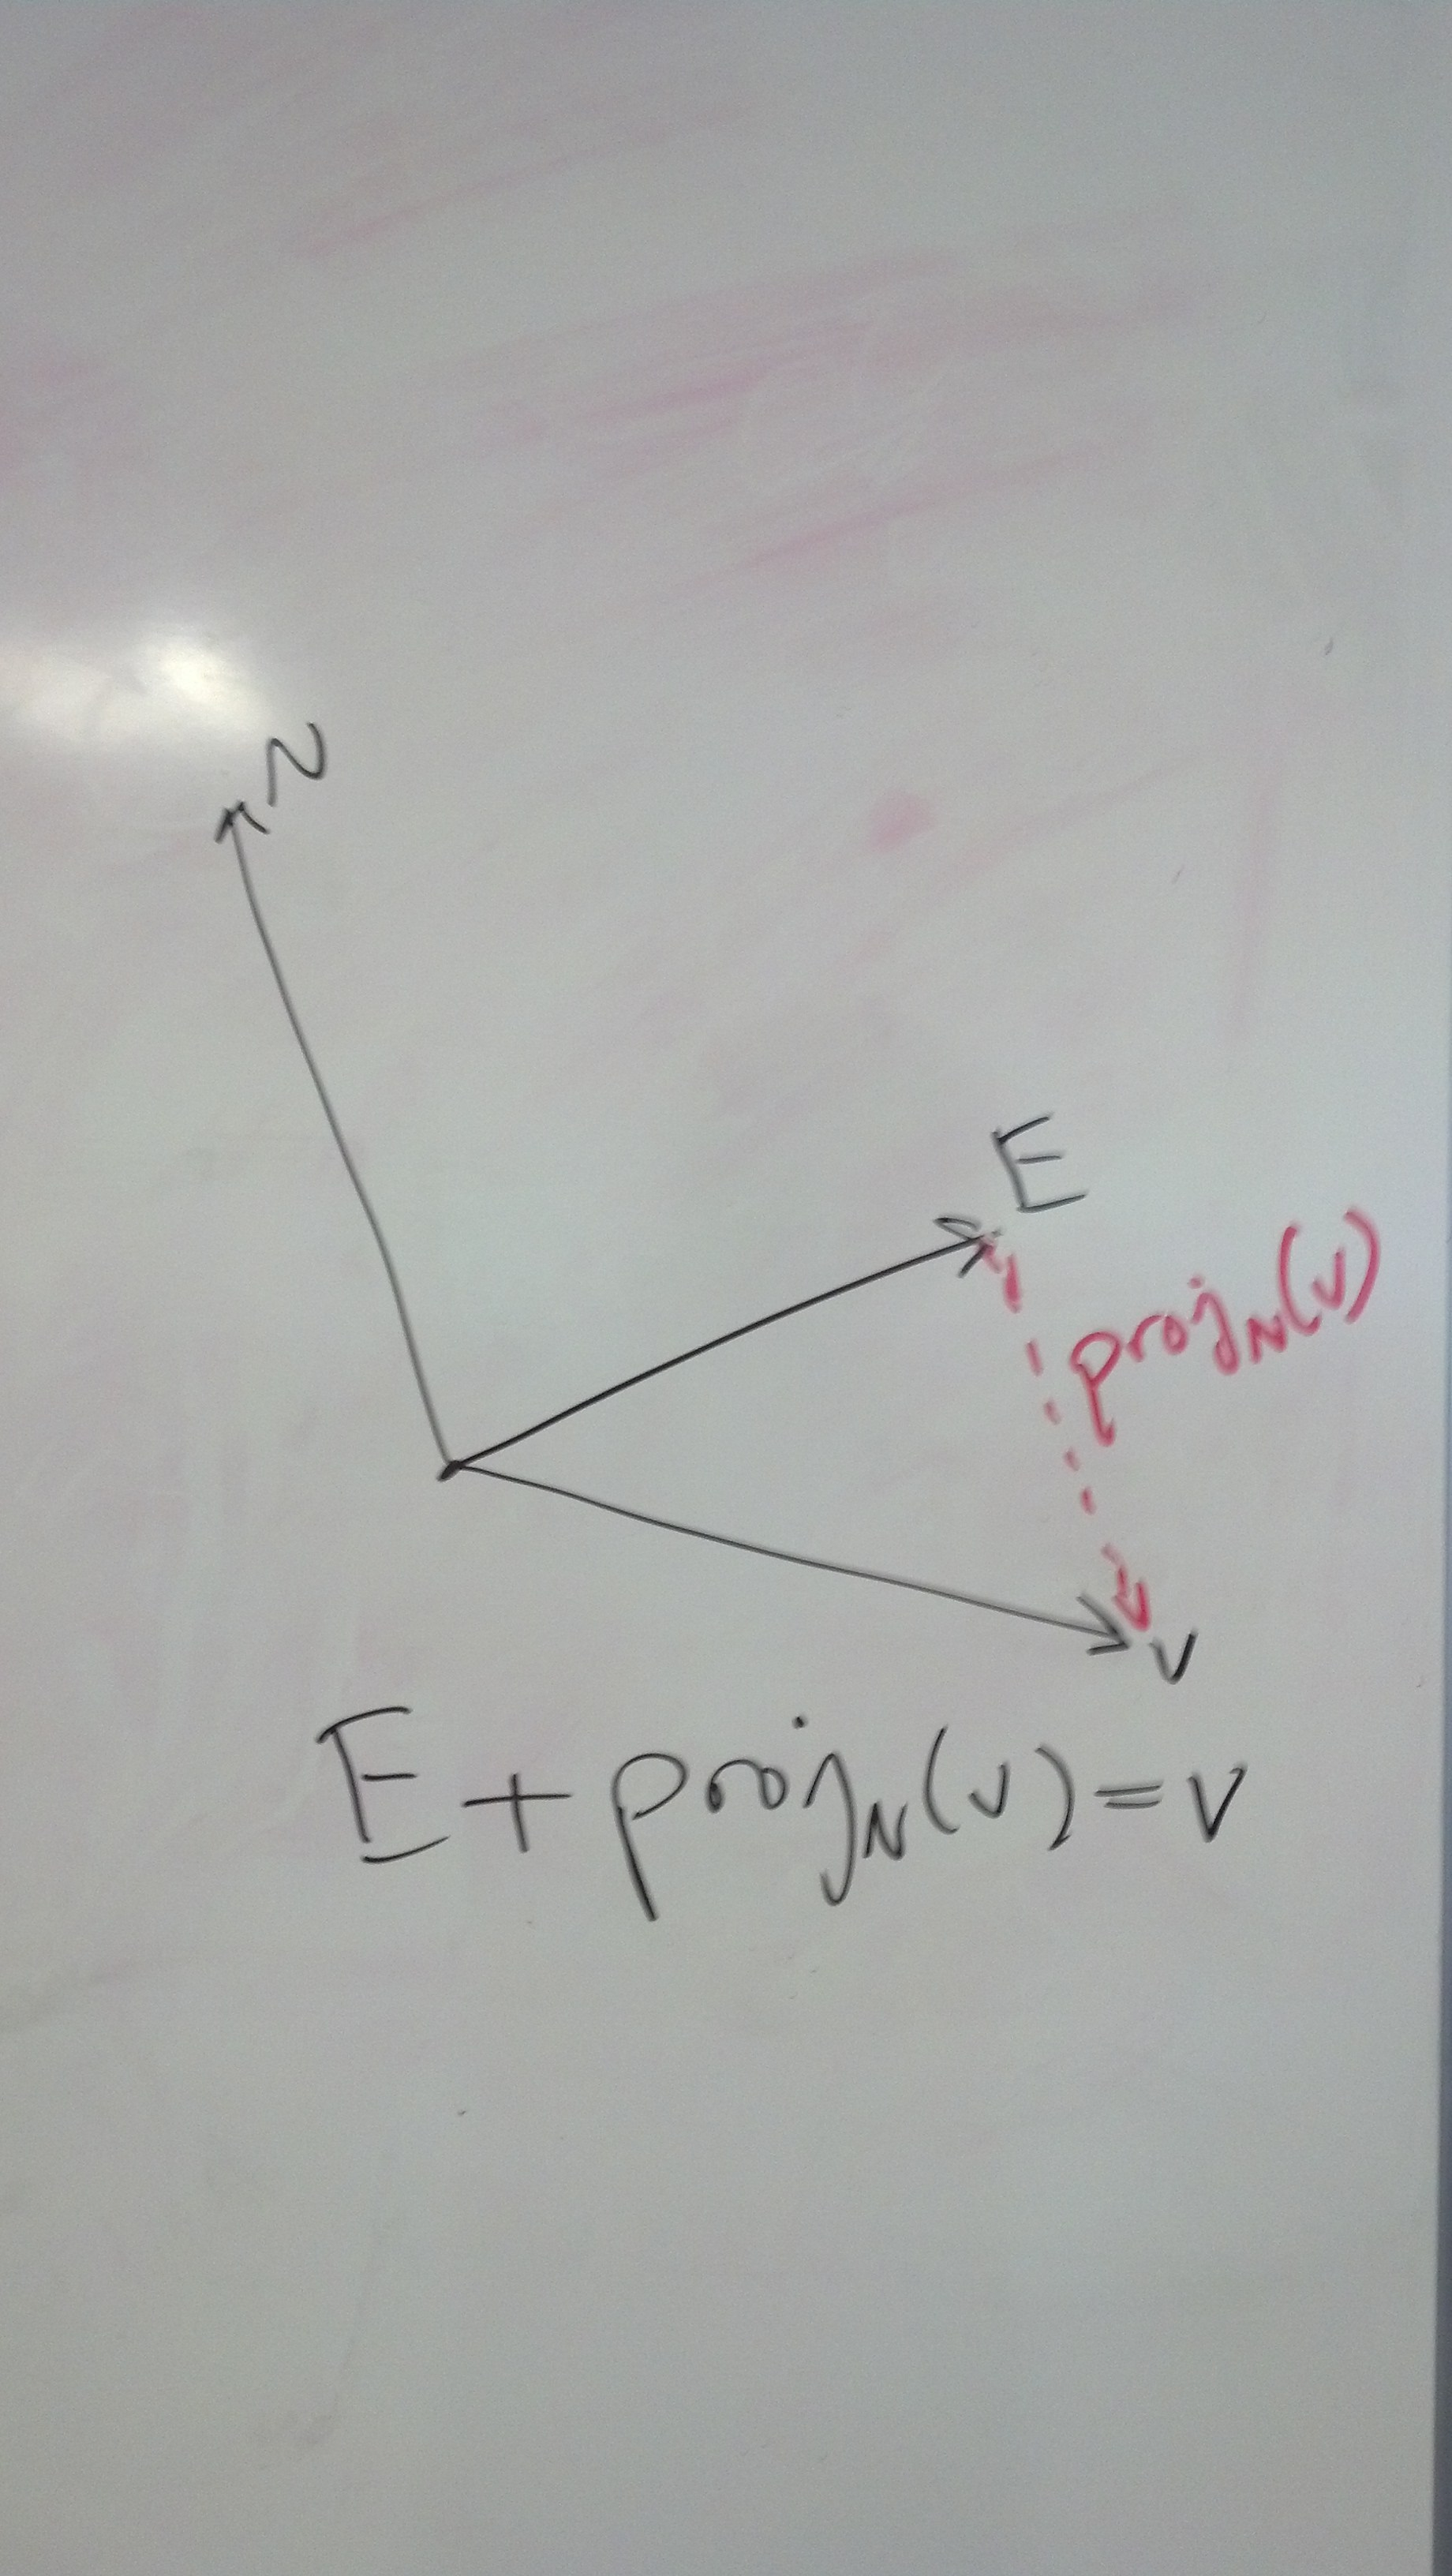
\includegraphics[width=\columnwidth]{vectordiagram.jpg}
\caption{The segment vector, normal, and projected vector}
\label{vectordiagram}
\end{figure}

Thus, the following equation will get us $E$
\[
E = v - proj_N(v)
\]
This can be further simplified to say
\[
E = v - N(v.N)
\]
We then find the intersection of the vector $E$ with the current triangle. If the segment is entirely in the triangle, then we move onto the next segment starting from the endpoint of $E$. If the segment leaves the triangle, then we find which edge the segment intersects and repeat the projection procedure for the end part of the segment that is not in the triangle. This procedure of course relied on finding the intersection of the triangle with the segment which proved to be non-trivial.\\
\\
When finding the triangle and segment intersection, we had a triangle in a 3D space as well as a segment that was supposed to be coplanar to the triangle but could be slightly off due to floating-point errors with the coordinates. To find the intersection point, I converted the segment and triangle coordinates to the coordinate system where one of the vertices of the triangle is the origin and the basis vectors are the two vectors made by the segments coming off that vertex as well as the cross product of those vectors. In this coordinate system, the third coordinate should be zero. In practice, it was near zero due to floating point errors. Once in the new coordinate system, we just had to find the 2D intersection of the triangle and the segment. \\
\\
The above procedure describes what we did with a single segment. With paths, we just iterated this procedure for each segment of the path. We assumed that the important aspect of each segment is its vector and not its origin point, since that is what we get from the probe. This meant that the end point of a projected segment was treated as the start point for the rest of the path when doing the loop to project the entire path onto the mesh.

\subsection{Justification}

%In Theorem 9.10.11 of \ref{mathText}, the geodesic is defined to be the curve of shortest %length between two points on the surface. 
We have a recorded path and an algorithm to transform that to the surface. Because a path is a series of short segments, we just need to justify that algorithm for a single segment. Each segment of our path represents the distance and direction traveled in a very small amount of time. We are given a start point on the surface and vector and need to calculate the path on the surface. \\
\\
This tracking system is meant to be used with a system that rapidly samples the location of a probe. This means that an individual segment is thus quite short. Additionally, the surface is generally assumed to a low curvature. The surface we are tracking over must be a manifold. The combination of short segments and low curvature leads to the following assertion that will be used in my justification: {\it If $\epsilon$ is the length of the segment, then the $\epsilon$-neighborhood around the start point of the segment is homeomorphic to $R^2$}. This is illustrated in figure \ref{manifolddiagram}.\\
\\
\begin{figure}[ht]
\centering
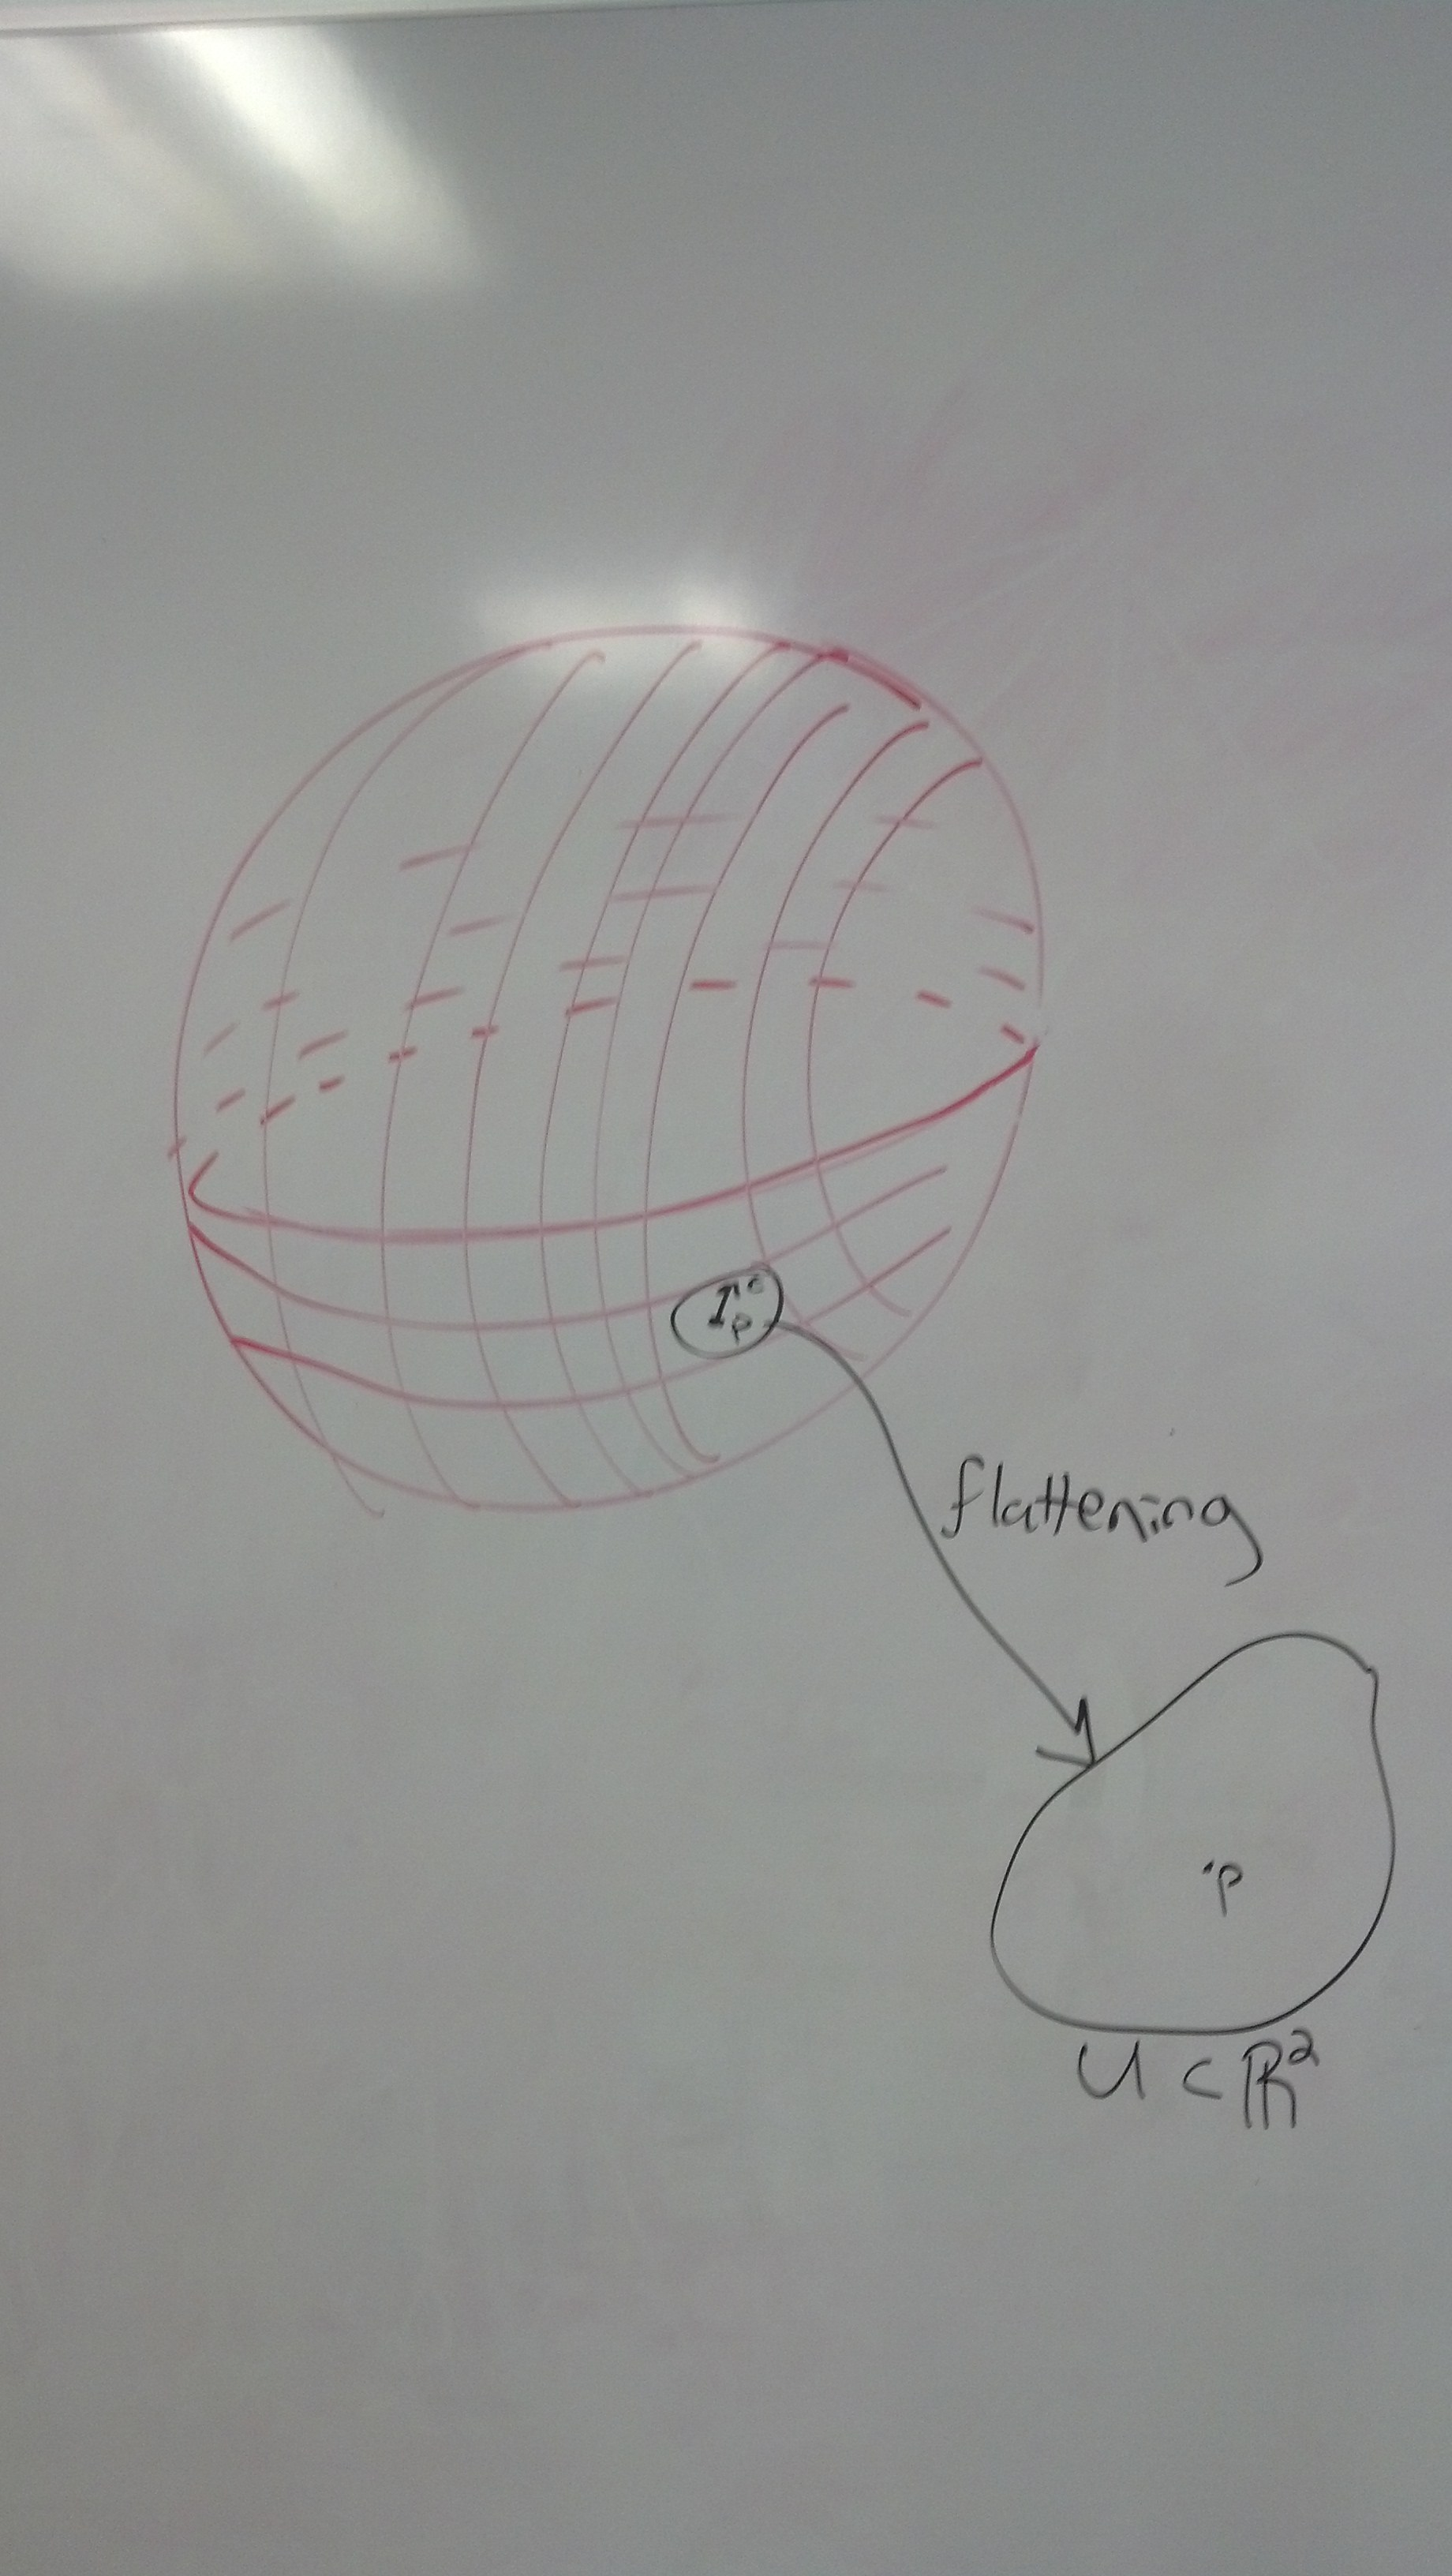
\includegraphics[width=\columnwidth]{manifolddiagram.jpg}
\caption{The manifold with its $\epsilon$ neighborhood at a point $p$}
\label{manifolddiagram}
\end{figure}
Because the sampling rate was so rapid, we can assert that between samples, a straight line on the surface was followed. We can thus assert the following: {\it The segment follows the geodesic path from start to end point along the surface}. We do not have the end point on the surface but when we assert an end point later, the path that was calculated will be the geodesic path from start to end point along the surface. \\
\\
At a given point, the probe is either on the surface or pressing into the surface in the direction of the normal to the surface. This is because when someone is guiding the probe, they are pressing {\it down} on the surface meaning that the pressing is in the direction of the normal. This allows us to assert the following: {\it The transformed segment vector must be perpendicular to the normal. }\\
\\
Because the rotation calibration step takes care of the orientation along the surface, we must transform our vector in such a way that preserves that. We thus assert that we can only rotate the vector in the plane formed by the segment vector and the normal. Rotating it in any other plane would change the orientation along the surface. The transformed vector still needs to be perpendicular to the normal, thus we will have two options for it. We must pick the option that leaves us with an acute angle between the transformed vector and original vector as picking the other one would also change the orientation. We have now justified the following facts that were used to make the formula for the transformed segment vector: \\
{\it The transformed vector must be rotated along the same plane as the normal and the original vector}\\
{\it The transformed vector and original vector must form an acute angle}
\\
\\
We have now justified the direction of our transformed vector. We need to preserve arc-length of the path hence the length of our transformed vector will be the same as the length of the segment vector. This could have the implication that the transformed vector goes past the triangle it is located on. If that is the case, then we cut off the segment at the edge and transform the remaining vector. We repeat this procedure until a segment lies entirely in a triangle. \\
\\
We finally need to justify that this produces the geodesic in our desired direction on the surface. In the case where the entire segment can be put into its current triangle, this is trivial as we are following the straight line along that part of the surface. We thus need to justify the case where we traverse multiple triangles. Due to the homeomorphism mentioned above, we can locally flatten the triangles and avoid the gaps and overlaps that sometimes happen when there is mesh flattening. At each point in the algorithm, we are putting the path on the plane in the direction of the segment. Thus it is in the straight line direction. This means that when you flatten the triangles, the path will be a straight line in the direction we wanted. It will thus be the shortest path between the start and end points. This is illustrated in figure \ref{flatteningDiagram_oneTriangle} and figure \ref{flatteningDiagram_neighborhood}. 
\begin{figure}[ht]
\centering
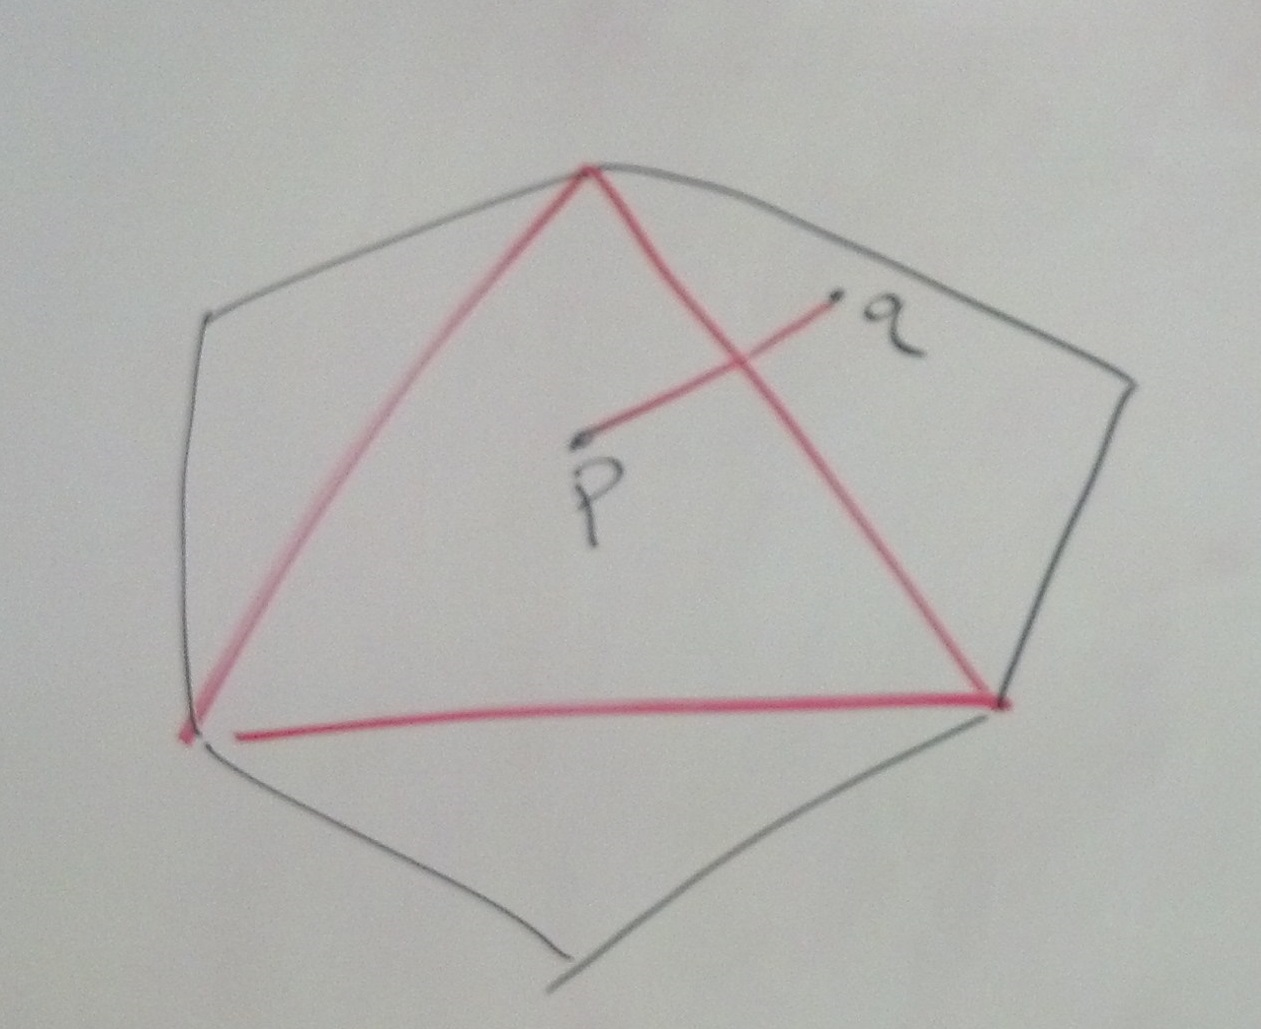
\includegraphics[width=\columnwidth]{flatteningdiagram_oneTriangleAndNeighbors.jpg}
\caption{The triangle at $p$ and its neighbors}
\label{flatteningDiagram_oneTriangle}
\end{figure}
\begin{figure}[ht]
\centering
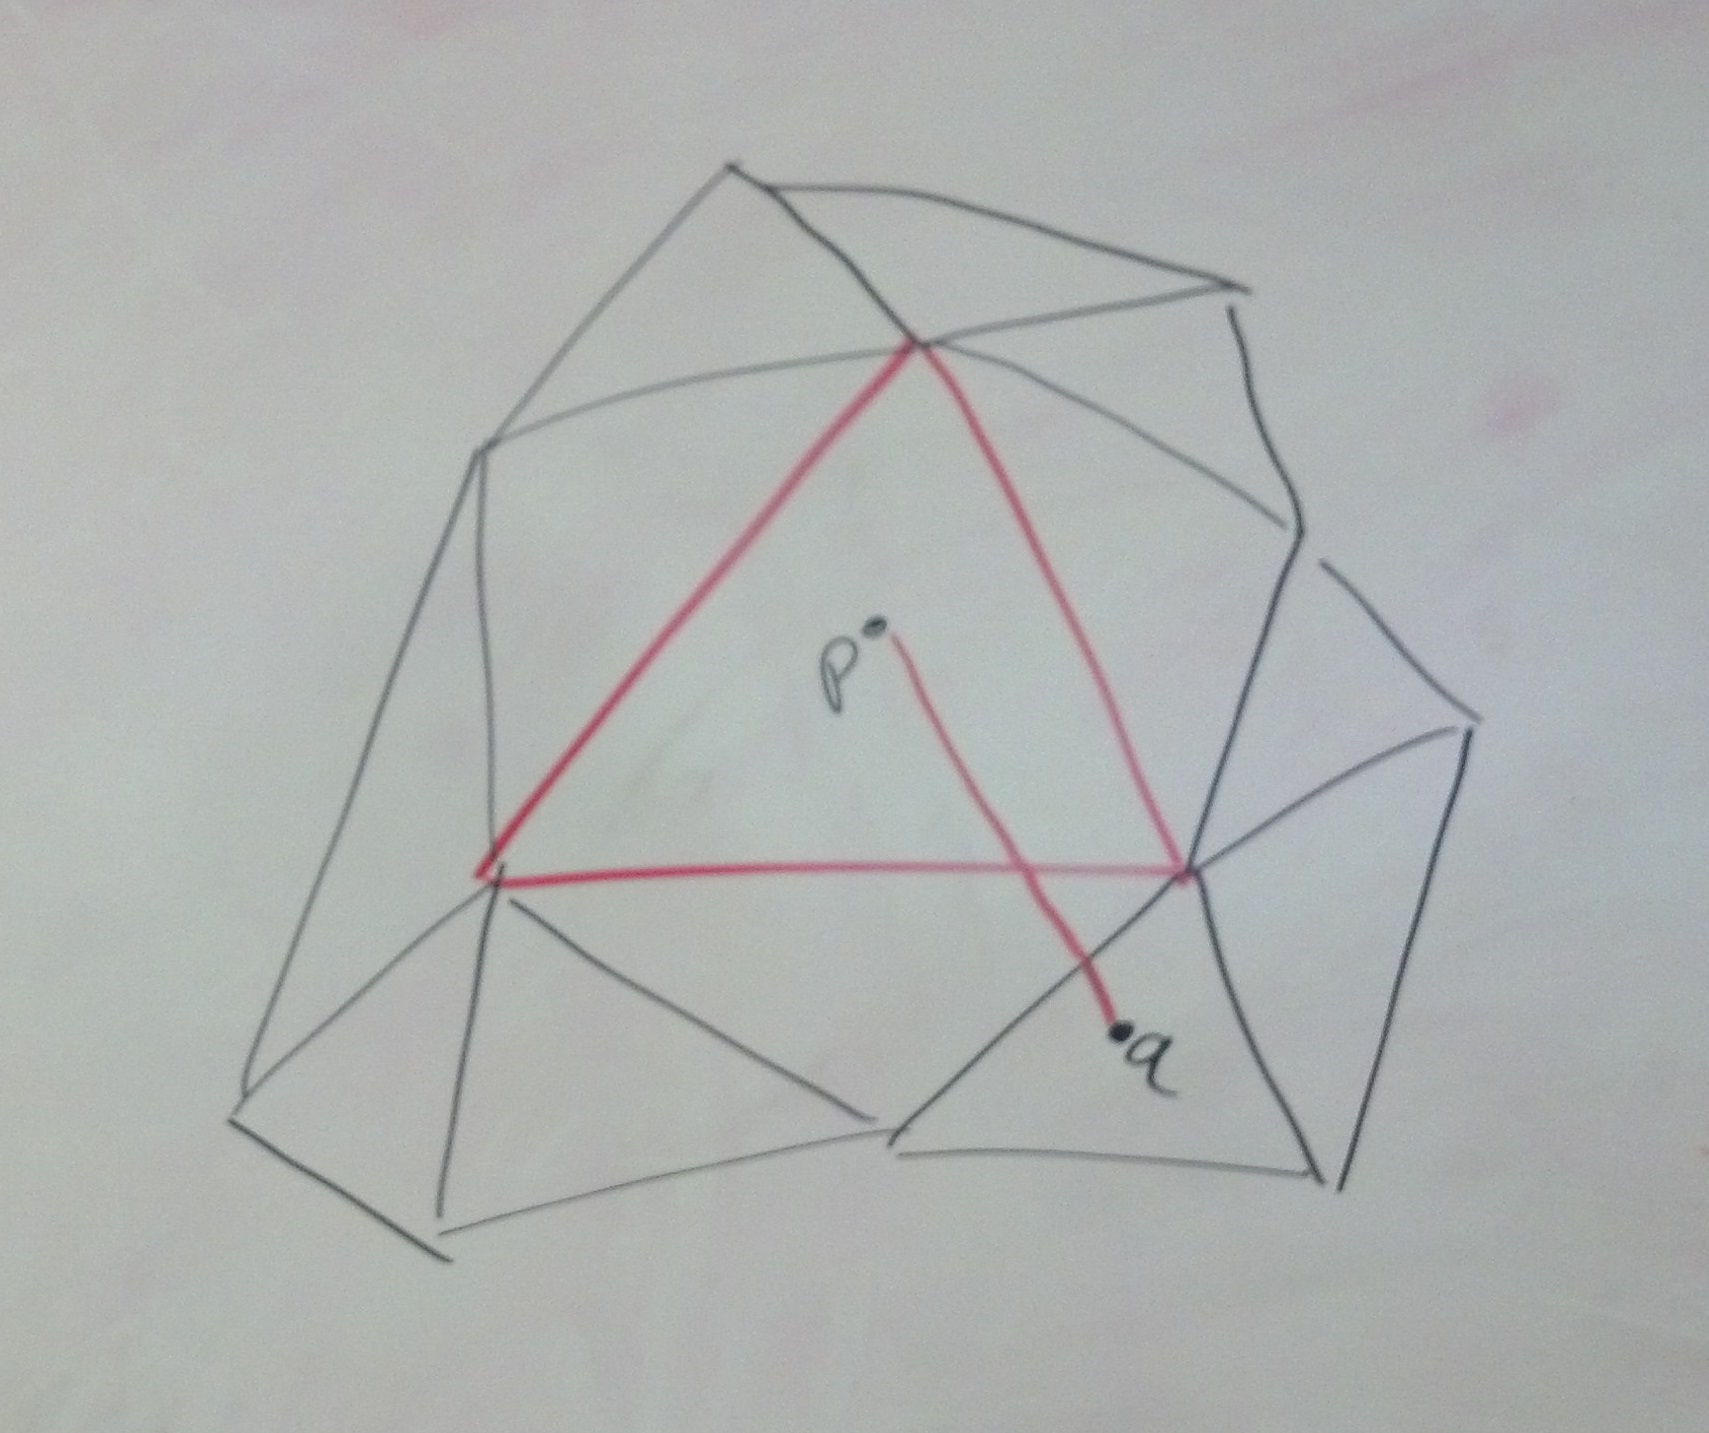
\includegraphics[width=\columnwidth]{flatteningdiagram_neighborhood.jpg}
\caption{The triangles in the neighborhood around $p$}
\label{flatteningDiagram_neighborhood}
\end{figure}




\bibliographystyle{acmsiggraph}
\bibliography{trackingRefs}

\end{document}
